% Method overview (Fig. 2), vector version. Compile standalone to figures/fig02_method.pdf.
% Role colours match figures/fig_target_coding.pdf (scripts/make_label_figures.py, ROLE palette).
\documentclass[tikz,border=2pt]{standalone}
\usepackage{fontspec}
\setmainfont{texgyreheros}[Extension=.otf, UprightFont=*-regular, BoldFont=*-bold,
  ItalicFont=*-italic, BoldItalicFont=*-bolditalic, Scale=0.95]
\usepackage{sansmath}
\usetikzlibrary{arrows.meta,calc,decorations.pathreplacing,positioning}
\definecolor{bg}{HTML}{D9D9D9}
\definecolor{ecs}{HTML}{C6DBEF}
\definecolor{pm}{HTML}{2171B5}
\definecolor{cyto}{HTML}{9ECAE1}
\definecolor{nucpl}{HTML}{6BAED6}
\definecolor{slotA}{HTML}{D95F02}
\definecolor{slotB}{HTML}{FDAE6B}
\definecolor{slotC}{HTML}{7F2704}
\definecolor{other}{HTML}{8E6BBF}
\definecolor{ink}{HTML}{222222}
\definecolor{soft}{HTML}{F3F3F1}
\definecolor{line}{HTML}{8A8A8A}
\tikzset{
  ch/.style={draw=white, line width=0.6pt, minimum width=0.92cm, minimum height=0.66cm, inner sep=0pt,
             font=\scriptsize, align=center, text=ink},
  dark/.style={text=white},
  box/.style={draw=line, fill=soft, rounded corners=2pt, text width=5.5cm, align=center,
               font=\scriptsize, inner sep=3pt, minimum height=0.62cm},
  arr/.style={-{Stealth[length=4pt]}, line width=0.6pt, color=ink},
  brace/.style={decorate, decoration={brace, amplitude=4pt}, line width=0.5pt, color=ink},
  ttl/.style={font=\footnotesize\bfseries, anchor=west, text=ink},
  note/.style={font=\scriptsize, text=ink, align=center},
}
% #1 y, #2 query label, #3-#5 slot texts, #6 style of slot 3, #7 node-name suffix
\newcommand{\chrow}[7]{%
  \node[font=\scriptsize, align=right, anchor=east, text=ink] at (2.15,#1) {#2};
  \node[ch, fill=bg]          (bg#7) at (2.76,#1) {BG};
  \node[ch, fill=ecs]         (a1#7) at (3.94,#1) {ecs};
  \node[ch, fill=pm, dark]    (a2#7) at (4.92,#1) {pm};
  \node[ch, fill=cyto]        (a3#7) at (5.90,#1) {cyto};
  \node[ch, fill=nucpl]       (a4#7) at (6.88,#1) {nucpl};
  \node[ch, fill=slotA, dark] (s1#7) at (8.06,#1) {#3};
  \node[ch, fill=slotB]       (s2#7) at (9.04,#1) {#4};
  \node[ch, #6]               (s3#7) at (10.02,#1) {#5};
  \node[ch, fill=other, dark] (o#7)  at (11.20,#1) {other\\FG};
}
\begin{document}
\hyphenpenalty=10000\exhyphenpenalty=10000
\begin{sansmath}
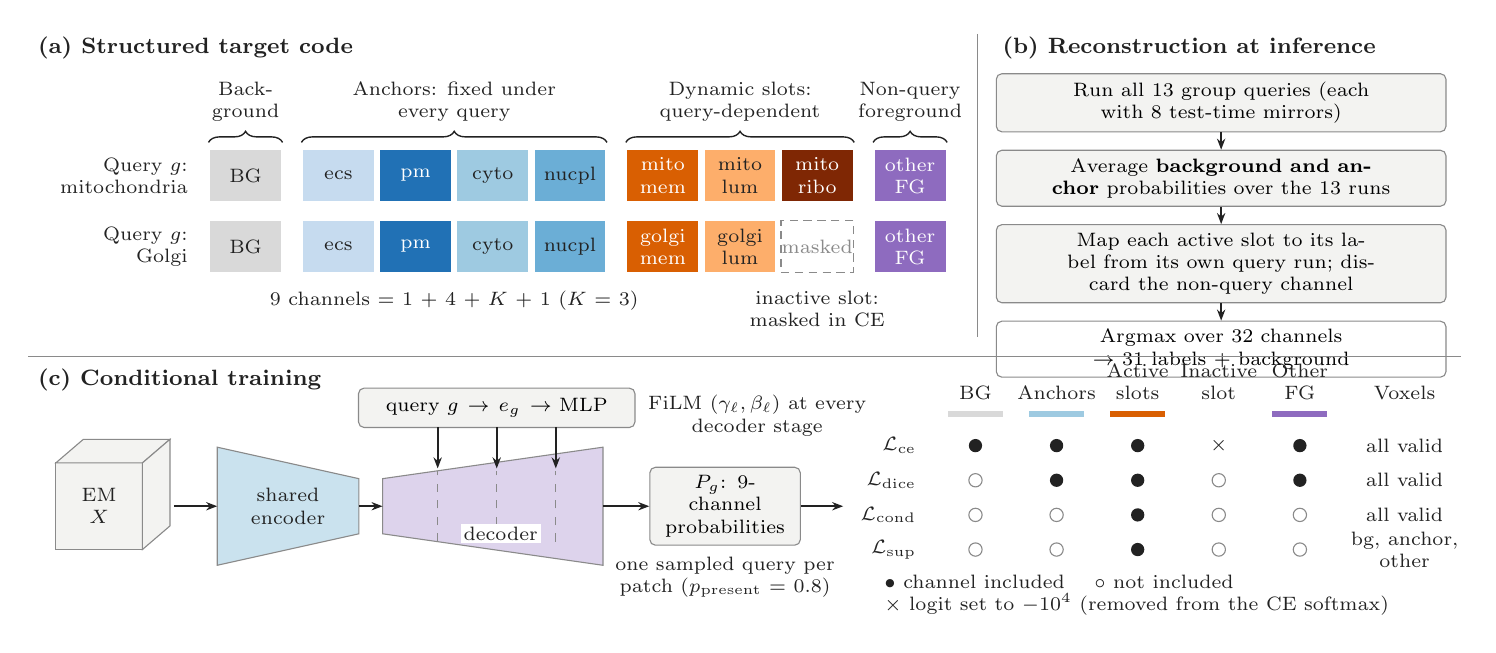
\begin{tikzpicture}[x=1cm, y=1cm]
% ---------------- (a) structured target code ----------------
\node[ttl] at (0,1.62) {(a) Structured target code};
\chrow{0}{Query $g$:\\mitochondria}{mito\\mem}{mito\\lum}{mito\\ribo}{fill=slotC, dark}{A}
\chrow{-0.9}{Query $g$:\\Golgi}{golgi\\mem}{golgi\\lum}{masked}{fill=white, draw=line, densely dashed, text=line}{B}
\draw[brace] ($(bgA.north west)+(0,0.08)$) -- ($(bgA.north east)+(0,0.08)$) node[midway, above=4pt, note] {Back-\\ground};
\draw[brace] ($(a1A.north west)+(0,0.08)$) -- ($(a4A.north east)+(0,0.08)$) node[midway, above=4pt, note] {Anchors: fixed under\\every query};
\draw[brace] ($(s1A.north west)+(0,0.08)$) -- ($(s3A.north east)+(0,0.08)$) node[midway, above=4pt, note] {Dynamic slots:\\query-dependent};
\draw[brace] ($(oA.north west)+(0,0.08)$) -- ($(oA.north east)+(0,0.08)$) node[midway, above=4pt, note] {Non-query\\foreground};
\node[note, anchor=north] at ($(s3B.south)+(0,-0.1)$) {inactive slot:\\masked in CE};
\node[note, anchor=north] at ($(a2B.south)!0.5!(a3B.south)+(0,-0.1)$) {9 channels = 1 + 4 + $K$ + 1 ($K$ = 3)};
% ---------------- (b) reconstruction ----------------
\draw[line, line width=0.4pt] (12.05,1.8) -- (12.05,-2.05);
\node[ttl] at (12.25,1.62) {(b) Reconstruction at inference};
\node[box, anchor=north] (r1) at (15.15,1.3) {Run all 13 group queries (each with 8 test-time mirrors)};
\node[box, below=0.22cm of r1] (r2) {Average \textbf{background and anchor} probabilities over the 13 runs};
\node[box, below=0.22cm of r2] (r3) {Map each active slot to its label from its own query run; discard the non-query channel};
\node[box, fill=white, below=0.22cm of r3] (r4) {Argmax over 32 channels $\rightarrow$ 31 labels + background};
\draw[arr] (r1) -- (r2); \draw[arr] (r2) -- (r3); \draw[arr] (r3) -- (r4);
% ---------------- (c) conditional training ----------------
\draw[line, line width=0.4pt] (0,-2.3) -- (18.2,-2.3);
\node[ttl] at (0,-2.6) {(c) Conditional training};
\begin{scope}[shift={(0.35,-4.75)}]
  \draw[fill=soft, draw=line] (0,0) rectangle (1.1,1.1);
  \draw[fill=soft, draw=line] (0,1.1) -- (0.35,1.4) -- (1.45,1.4) -- (1.1,1.1) -- cycle;
  \draw[fill=soft, draw=line] (1.1,0) -- (1.45,0.3) -- (1.45,1.4) -- (1.1,1.1) -- cycle;
  \node[note] at (0.55,0.55) {EM\\$X$};
\end{scope}
\draw[fill=cyto!55, draw=line] (2.4,-4.95) -- (4.2,-4.55) -- (4.2,-3.85) -- (2.4,-3.45) -- cycle;
\node[note] at (3.3,-4.2) {shared\\encoder};
\draw[fill=other!30, draw=line] (4.5,-4.55) -- (7.3,-4.95) -- (7.3,-3.45) -- (4.5,-3.85) -- cycle;
\foreach \x in {5.2,5.95,6.7} { \draw[line, dashed, line width=0.4pt] (\x,-4.65) -- (\x,-3.75); }
\node[note, fill=white, inner sep=1pt] at (6.0,-4.55) {decoder};
\draw[arr] (1.85,-4.2) -- (2.4,-4.2);
\draw[arr] (4.2,-4.2) -- (4.5,-4.2);
\node[box, text width=3.3cm, minimum height=0.5cm] (q) at (5.95,-2.95) {query $g \rightarrow e_g \rightarrow$ MLP};
\foreach \x in {5.2,5.95,6.7} { \draw[arr] (\x,-3.2) -- (\x,-3.72); }
\node[note, anchor=west] at (7.75,-3.05) {FiLM $(\gamma_\ell,\beta_\ell)$ at every\\decoder stage};
\node[box, text width=1.7cm] (p) at (8.85,-4.2) {$P_g$: 9-channel\\probabilities};
\draw[arr] (7.3,-4.2) -- (p.west);
\node[note] at (8.85,-5.1) {one sampled query per\\patch ($p_{\mathrm{present}}$ = 0.8)};
\draw[arr] (p.east) -- (10.35,-4.2);
% loss coverage: rows are loss terms, columns are output channels
\begin{scope}[shift={(10.45,-3.05)}]
  \def\cw{1.03}
  \def\mm{m}
  \foreach \lab/\col/\i in {BG/bg/1, Anchors/cyto/2, {Active\\slots}/slotA/3, {Inactive\\slot}/white/4, {Other\\FG}/other/5} {
    \node[note, anchor=south] at (\i*\cw+0.55,0.08) {\lab};
    \fill[\col] (\i*\cw+0.2,-0.02) rectangle (\i*\cw+0.9,0.06);
  }
  \node[note, anchor=south] at (6*\cw+0.85,0.08) {Voxels};
  \foreach \name/\r in {{$\mathcal{L}_{\mathrm{ce}}$}/1, {$\mathcal{L}_{\mathrm{dice}}$}/2, {$\mathcal{L}_{\mathrm{cond}}$}/3, {$\mathcal{L}_{\mathrm{sup}}$}/4} {
    \node[note, anchor=east] at (0.95,-\r*0.44+0.06) {\name};
  }
  % 1 = channel included, 0 = not included, m = removed from the CE softmax
  \foreach \row/\cells/\vox in {1/{1,1,1,m,1}/{all valid}, 2/{0,1,1,0,1}/{all valid}, 3/{0,0,1,0,0}/{all valid}, 4/{0,0,1,0,0}/{bg, anchor,\\other}} {
    \foreach \v [count=\c] in \cells {
      \coordinate (cc) at (\c*\cw+0.55,-\row*0.44+0.06);
      \ifx\v\mm \node[font=\scriptsize, text=ink] at (cc) {$\times$};
      \else \ifnum\v=1 \fill[ink] (cc) circle (2.4pt); \else \draw[line] (cc) circle (2.4pt); \fi \fi
    }
    \node[note] at (6*\cw+0.85,-\row*0.44+0.06) {\vox};
  }
  \node[note, anchor=north west, align=left] at (0.3,-1.9)
    {$\bullet$ channel included \quad $\circ$ not included\\$\times$ logit set to $-$10\textsuperscript{4} (removed from the CE softmax)};
\end{scope}
\end{tikzpicture}
\end{sansmath}
\end{document}
